\newpage
\section{Drivers}
\subsection{Environnement Qemu et plate-forme Reptar }
Lors de cette étape, nous allons déployer l'environnement de la cible à partir d'une image de carte MMC
(sdcard) et nous nous familiariserons avec l'insertion dynamique de module.
Le projet concerné est le projet drivers (répertoire du même nom à la racine du workspace). \\\\
\textbf{a) Donnée: }Lancez make dans le répertoire drivers/\\\\
\textbf{Travail réalisé: }
\begin{lstlisting}
$ cd ~/seee_student/drivers/
$ make
...
make[1]: Leaving directory `/home/redsuser/seee_student/linux-3.0-reptar'
arm-linux-gnueabihf-gcc -marm -I../linux-3.0-reptar -static buttons_test.c -o buttons_test
$
\end{lstlisting}
\textbf{b) Donnée: }A la racine du workspace, lancez les scripts suivants, puis la commande boot dans U-boot :
\begin{lstlisting}
$ ./deploy
$ ./stf
Reptar # boot 
\end{lstlisting}
\textbf{Travail réalisé: }
\begin{lstlisting}
$ cd ~/seee_student/drivers
$ ./deploy 
Deploying into reptar rootfs ...
Mounting filesystem/sd-card.img...
[sudo] password for redsuser: 
SD card partitions mounted in 'boot_tmp' and 'filesystem_tmp' directories
Unmounting SD card image...
Synchronizing .img file
Unmounting 'boot_tmp' and 'filesystem_tmp'...
Done !
$ ./stf
...
Reptar # boot
reading uImage
...
*** Welcome on REPTAR (HEIG-VD/REDS): use root/root to log in ***
reptar login: root
Password: 
# 
\end{lstlisting}
\textbf{c) Donnée: }A la racine du rootfs (cd /), insérez le module avec la commande suivante :
\begin{lstlisting}
# insmod sp6.ko 
\end{lstlisting}
Vérifiez qu'il n'y ait aucun message d'erreur. La liste des modules chargés dynamiquement est obtenue
avec la commande lsmod et le retrait du module avec la commande rmmod 
\begin{lstlisting}
# lsmod
# rmmod sp6
reptar_sp6: bye bye!
# 
\end{lstlisting}
\textbf{Travail réalisé: }Avec la commande lsmod, on peut vérifier que notre module est correctement chargé. Si on le retire, il n'apparaît plus dans la liste.
\begin{lstlisting}
# cd /
# pwd
/
# insmod sp6.ko
reptar_sp6: module starting...
Probing FPGA driver (device: fpga)
input: reptar_sp6_buttons as /devices/platform/fpga/reptar_sp6_buttons/input/input1
reptar_sp6: done.
# lsmod
Module                  Size  Used by    Not tainted
sp6                     4606  0 
# rmmod sp6
reptar_sp6: bye bye!
# lsmod
Module                  Size  Used by    Not tainted
# 
\end{lstlisting}
\subsection{Driver de type caractère}
Cette étape consiste à travailler sur un driver de type caractère au niveau FPGA. Le code de cette
partie se trouve dans les fichiers reptar\_sp6.h et reptar\_sp6.c.
Sur la base du code existant, on souhaite pouvoir écrire et lire une chaîne de caractères contenant la
version du bitstream (hypothétique) dans la FPGA, stockée dans la variable globale bitstream\_version.\\\\
\textbf{a) Donnée: }Complétez les callbacks read() et write() afin qu'une application utilisateur puisse lire et écrire une
chaîne de (80 max.) caractères. \\\\
\textbf{Travail réalisé: }Les callbacks read et write ont été implémentés très sommairement dans le module avec la fonction 
\textit{copy\_from/to\_user}. Il faut faire attention à bien retourner le nombre de bytes qui ont été lus ou écrits, pour que l'application puisse être au fait et détecter le cas échéant, si une erreur s'est produite.\\
\begin{lstlisting}
# cd /
# insmod sp6.ko 
reptar_sp6: module starting...
Probing FPGA driver (device: fpga)
input: reptar_sp6_buttons as /devices/platform/fpga/reptar_sp6_buttons/input/input1
reptar_sp6: done.
# ./usertest 
Device ID : 0
Inode number : 5
Protection mode : 0
Num of hard links : 680
User ID of owner : 8624
Group ID of owner : 1
Device ID (spec files only): 0
Total size [bytes] : 0
Setting bitstream version to : mais coucou mon petit                                                          
Device ID : 0
Inode number : 5
Protection mode : 0
Num of hard links : 680
User ID of owner : 8624
Group ID of owner : 1
Device ID (spec files only): 0
Total size [bytes] : 0
Normally read buffer
Bitstream version : mais coucou mon petit
\end{lstlisting}

\textbf{b) Donnée: }Pour identifier le nom de l'entrée dans /dev/ qui sera créée automatiquement, examinez la fonction
probe( ) du driver.\\\\
\textbf{Réponse aux questions: }
\begin{enumerate}
	\item Comment l'entrée dans /dev est-elle générée ? 
	\item  Quel sera le nom de l'entrée dans /dev ? \\
\end{enumerate}
\textbf{Travail réalisé: }\\\\
\textbf{c) Donnée: }Afin de tester votre driver, écrivez une application usertest (fichier usertest.c) qui écrira puis relira
la chaîne de version en utilisant l’entrée dans /dev évoquée ci-dessus.\\
Une application a aussi été codée pour tester les callbacks. Celle-ci affiche les stats du fichier créé dans le dossier \textit{/dev}, écrit une version de bitstream totalement fabuliste, relit les stats et enfin lit le bitstream pour confirmer le succès de l'écriture.\\\\
\textbf{Réponse aux questions: }
\begin{enumerate}
	\item Recherchez les valeurs du major et minor attribuées à ce driver. Expliquez votre démarche\\
\end{enumerate}
\textbf{Travail réalisé: }\\\\
\subsection{Pilotage des LEDs }
Le code de pilotage des LEDs se trouve dans le fichier reptar\_sp6\_leds.c. La réalisation du driver des
LEDs.
\begin{enumerate}
	\item L’application graphique qtemu sera utilisée pour l'environnement émulé.
	\item Le driver devra être également testé sur la plate-forme réelle.
\end{enumerate}
Pour le pilotage des LEDs, on souhaite utiliser le sous-système leds présent dans le noyau Linux.
Effectuez un mappage du registre des LEDs à l'aide de la fonction ioremap( ), en vous servant de la
structure fpga\_resource.\\\\
\textbf{a) Donnée: }Enregistrez le device comme un device de type leds à l'aide de la fonction led\_classdev\_register( ).\\\\
\textbf{Emplacement du code: }\textit{Drivers/pilotageLeds/reptar\_sp6\_leds.c}\\\\
\textbf{Travail réalisé: }Nous avons modifié le fichier \textit{reptar\_sp6\_leds.c}. Avant de pouvoir enregistrer le device, il faut mapper le registre des LEDs avec la fonction \textit{ioremap}. Puis, on peut enregistrer le device comme ci-dessous:
\begin{lstlisting}
/* Map the LED register */
led->reg = ioremap(fpga_resource->start+pdata->reg_offset,2);

/* Register our new led device into led class */
led_classdev_register(&pdev->dev.parent, &led->cdev);
\end{lstlisting}
\textbf{b) Donnée: }Cherchez et implémentez le(s) callback(s) gérant l'enclenchement/déclenchement des LEDs.\\\\
\textbf{Travail réalisé: }En regardant dans la fonction \textit{probe}, on voit que le callback pour enregistrer les LEDs a été lié avec la fonction \textit{reptar\_sp6\_led\_set}.
\begin{lstlisting}
led->cdev.brightness_set = reptar_sp6_led_set;
led->cdev.name = pdata->name;
\end{lstlisting}
Pour interagir avec l'état des LEDs, il nous suffit de modifier la valeur du registre que l'on a précédent mapper avec \textit{ioremap}. On accède directement au périphérique. La modification du registre est protégée par un \textit{spin\_lock} pour gérer l'accès concurrent, car le registre est partagé.
\begin{lstlisting}
/* Protect access to shared register */
spin_lock(&reg_lock);

/* to be completed */
if(value)
*led->reg |= 0x0001 << (pd->bit);
else
*led->reg &= ~ (0x0001 << (pd->bit));
spin_unlock(&reg_lock);
\end{lstlisting}
\textbf{Réponse aux questions: }
\begin{enumerate}
	\item Combien y a-t-il de devices de type LED gérés par notre driver ?\\
\end{enumerate}
Il y a 6 LEDs selon la déclaration dans reptar\_sp6.h et il y a bien 6 LEDs dans la structure reptar\_sp6\_leds\_pdata[] du fichier reptar\_sp6.h
\begin{lstlisting}
/* Only LEDS 0 to 5 are under CPU control. 6 and 7 are used by the FPGA itself */
#define SP6_NUM_LEDS 6
\end{lstlisting}
\textbf{c) Donnée: }Testez le driver LED dans l'environnement qtemu (application graphique). Lancez le script
ledstest.sh.\\\\
\textbf{Travail réalisé: }Pour tester le driver dans l'émulateur, il ne faut plus travailler dans l'U-boot, mais dans Linux. Pour cela, il faut entrer la commande \textit{boot} au démarrage de l'émulateur. Le script \textit{ledstest.sh} peut être lancé une fois le driver inséré dans le noyau avec la commande \textit{insmod}. On peut ensuite suivre la séquence d'allumage/extinction des LEDs dans la représentation graphique \textit{qtemu}.
\begin{lstlisting}
$ cd ~/seee_student/drivers/
$ make
...
make[1]: Leaving directory /home/redsuser/seee_student/linux-3.0-reptar
$ cd ..
$ ./deploy
...
Done !
$ ./stq
...

Reptar # boot
...
*** Welcome on REPTAR (HEIG-VD/REDS): use root/root to log in ***
reptar login: root
Password: 

# cd /
# insmod sp6.ko 
reptar_sp6: module starting...
Probing FPGA driver (device: fpga)
input: reptar_sp6_buttons as /devices/platform/fpga/reptar_sp6_buttons/input/input1
reptar_sp6: done.

# ./ledstest.sh 
SP6 leds present in sysfs !
Turning on LEDS from right to left...
sp6_read: Led read 0x0
sp6_write: Led write 0x1
reptar-sp6-emul: sp6_emul_cmd_post
reptar-sp6-emul: sp6_emul_cmd_post Inserting into queue...
reptar-sp6-emul: sp6_emul_cmd_post ...done
sp6_read: Led read 0x1
sp6_write: Led write 0x3
reptar-sp6-emul: sp6_emul_cmd_post
reptar-sp6-emul: sp6_emul_cmd_post Inserting into queue...
reptar-sp6-emul: sp6_emul_cmd_post ...done
sp6_read: Led read 0x3
...
End of test
\end{lstlisting}
L'image ci-dessous montre que l'on arrive à piloter les LEDs
\begin{figure}[H]
	\begin{center}
		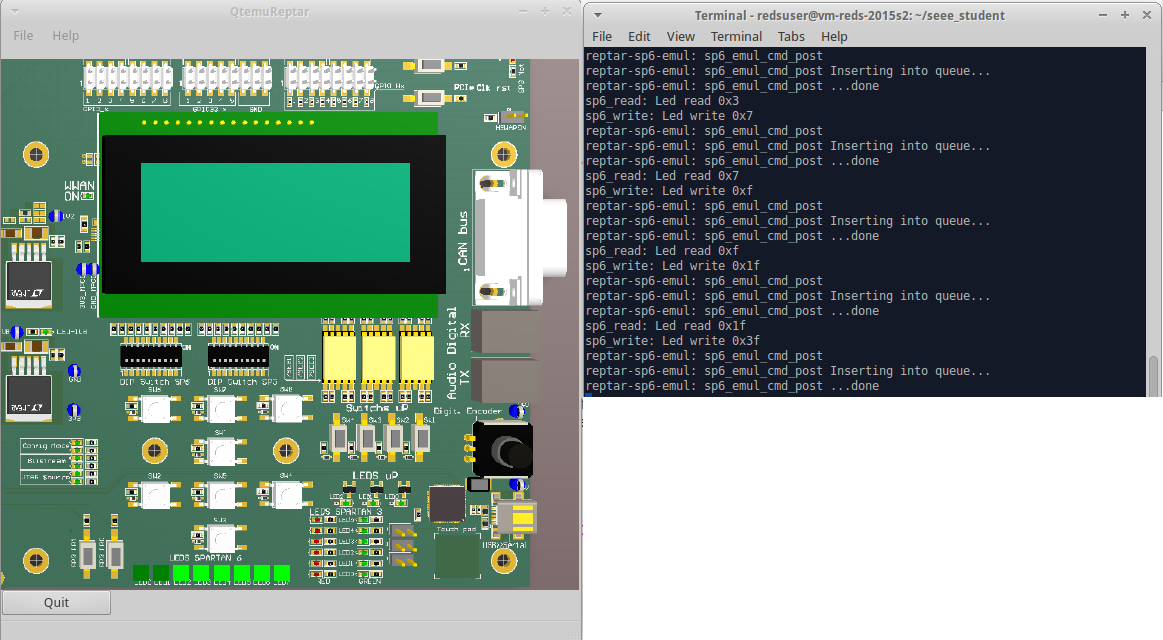
\includegraphics[width=17cm]{img/driverLeds.png}
		\caption{Test du pilote des LEDs avec qtemu}
		\label{driverLed3}
	\end{center}
\end{figure}
\textbf{d) Donnée: }Testez votre driver sur la plate-forme (réelle) Reptar.\\\\
\textbf{Travail réalisé: }Pour le test sur la plateforme réelle, nous avons également besoin de travailler dans Linux, on doit donc insérer la carte SD où se trouve l'image du noyau dans la plateforme, sans quoi on ne pourra pas booter. Nous avons remarqué que l'adresse IP de la carte Reptar avait encore changé. Maintenant c'est l'adresse 192.168.1.10.
\begin{lstlisting}
$ sudo picocom -b 115200 /dev/ttyUSB0 
[sudo] password for redsuser: 
picocom v1.7
...
Terminal ready

Reptar # boot
...
*** Welcome on REPTAR (HEIG-VD/REDS): use root/root to log in ***
reptar login: root
Password: 
# ifconfig
eth0      Link encap:Ethernet  HWaddr E4:AF:A1:40:01:0A  
inet addr:192.168.1.10  Bcast:192.168.1.255  Mask:255.255.255.0
...
\end{lstlisting}
Depuis la machine hôte, on va transférer par la connexion réseau les fichiers ledstest.sh et sp6.ko nécessaire. Nous avons besoin pour cela de la commande scp et de l'adresse IP de la plateforme
\begin{lstlisting}
$ cd ~/seee_student/drivers/
$ scp ledstest.sh root@192.168.1.10:ledstest.sh
root@192.168.1.10's password: 
ledstest.sh                                   100%  772     0.8KB/s   00:00  
  
$ scp sp6.ko root@192.168.1.10:sp6.ko
root@192.168.1.10's password: 
sp6.ko                                        100%  161KB 161.1KB/s   00:00    
\end{lstlisting}
Une fois les fichiers copiés, on accède à la plateforme par la connexion série et l'on peut installer notre driver et lancer le script de tests.
\begin{lstlisting}
# ls
bitstreams   helloworld   ledstest.sh  sp6.ko       tests
# insmod sp6.ko 
reptar_sp6: module starting...
Probing FPGA driver (device: fpga)
input: reptar_sp6_buttons as /devices/platform/fpga/reptar_sp6_buttons/input/input2
reptar_sp6: done.
# ./ledstest.sh 
SP6 leds present in sysfs !
Turning on LEDS from right to left...
Turning off LEDS from right to left...
All LEDS ON...
All LEDS OFF...
End of test
# rmmod sp6.ko 
reptar_sp6: bye bye!
\end{lstlisting}
Les images ci-dessous prouvent le bon fonctionnement de notre pilote des LEDs. On voit qu'elles s'allument et s'éteignent.
\begin{figure}[H]
	\begin{center}
		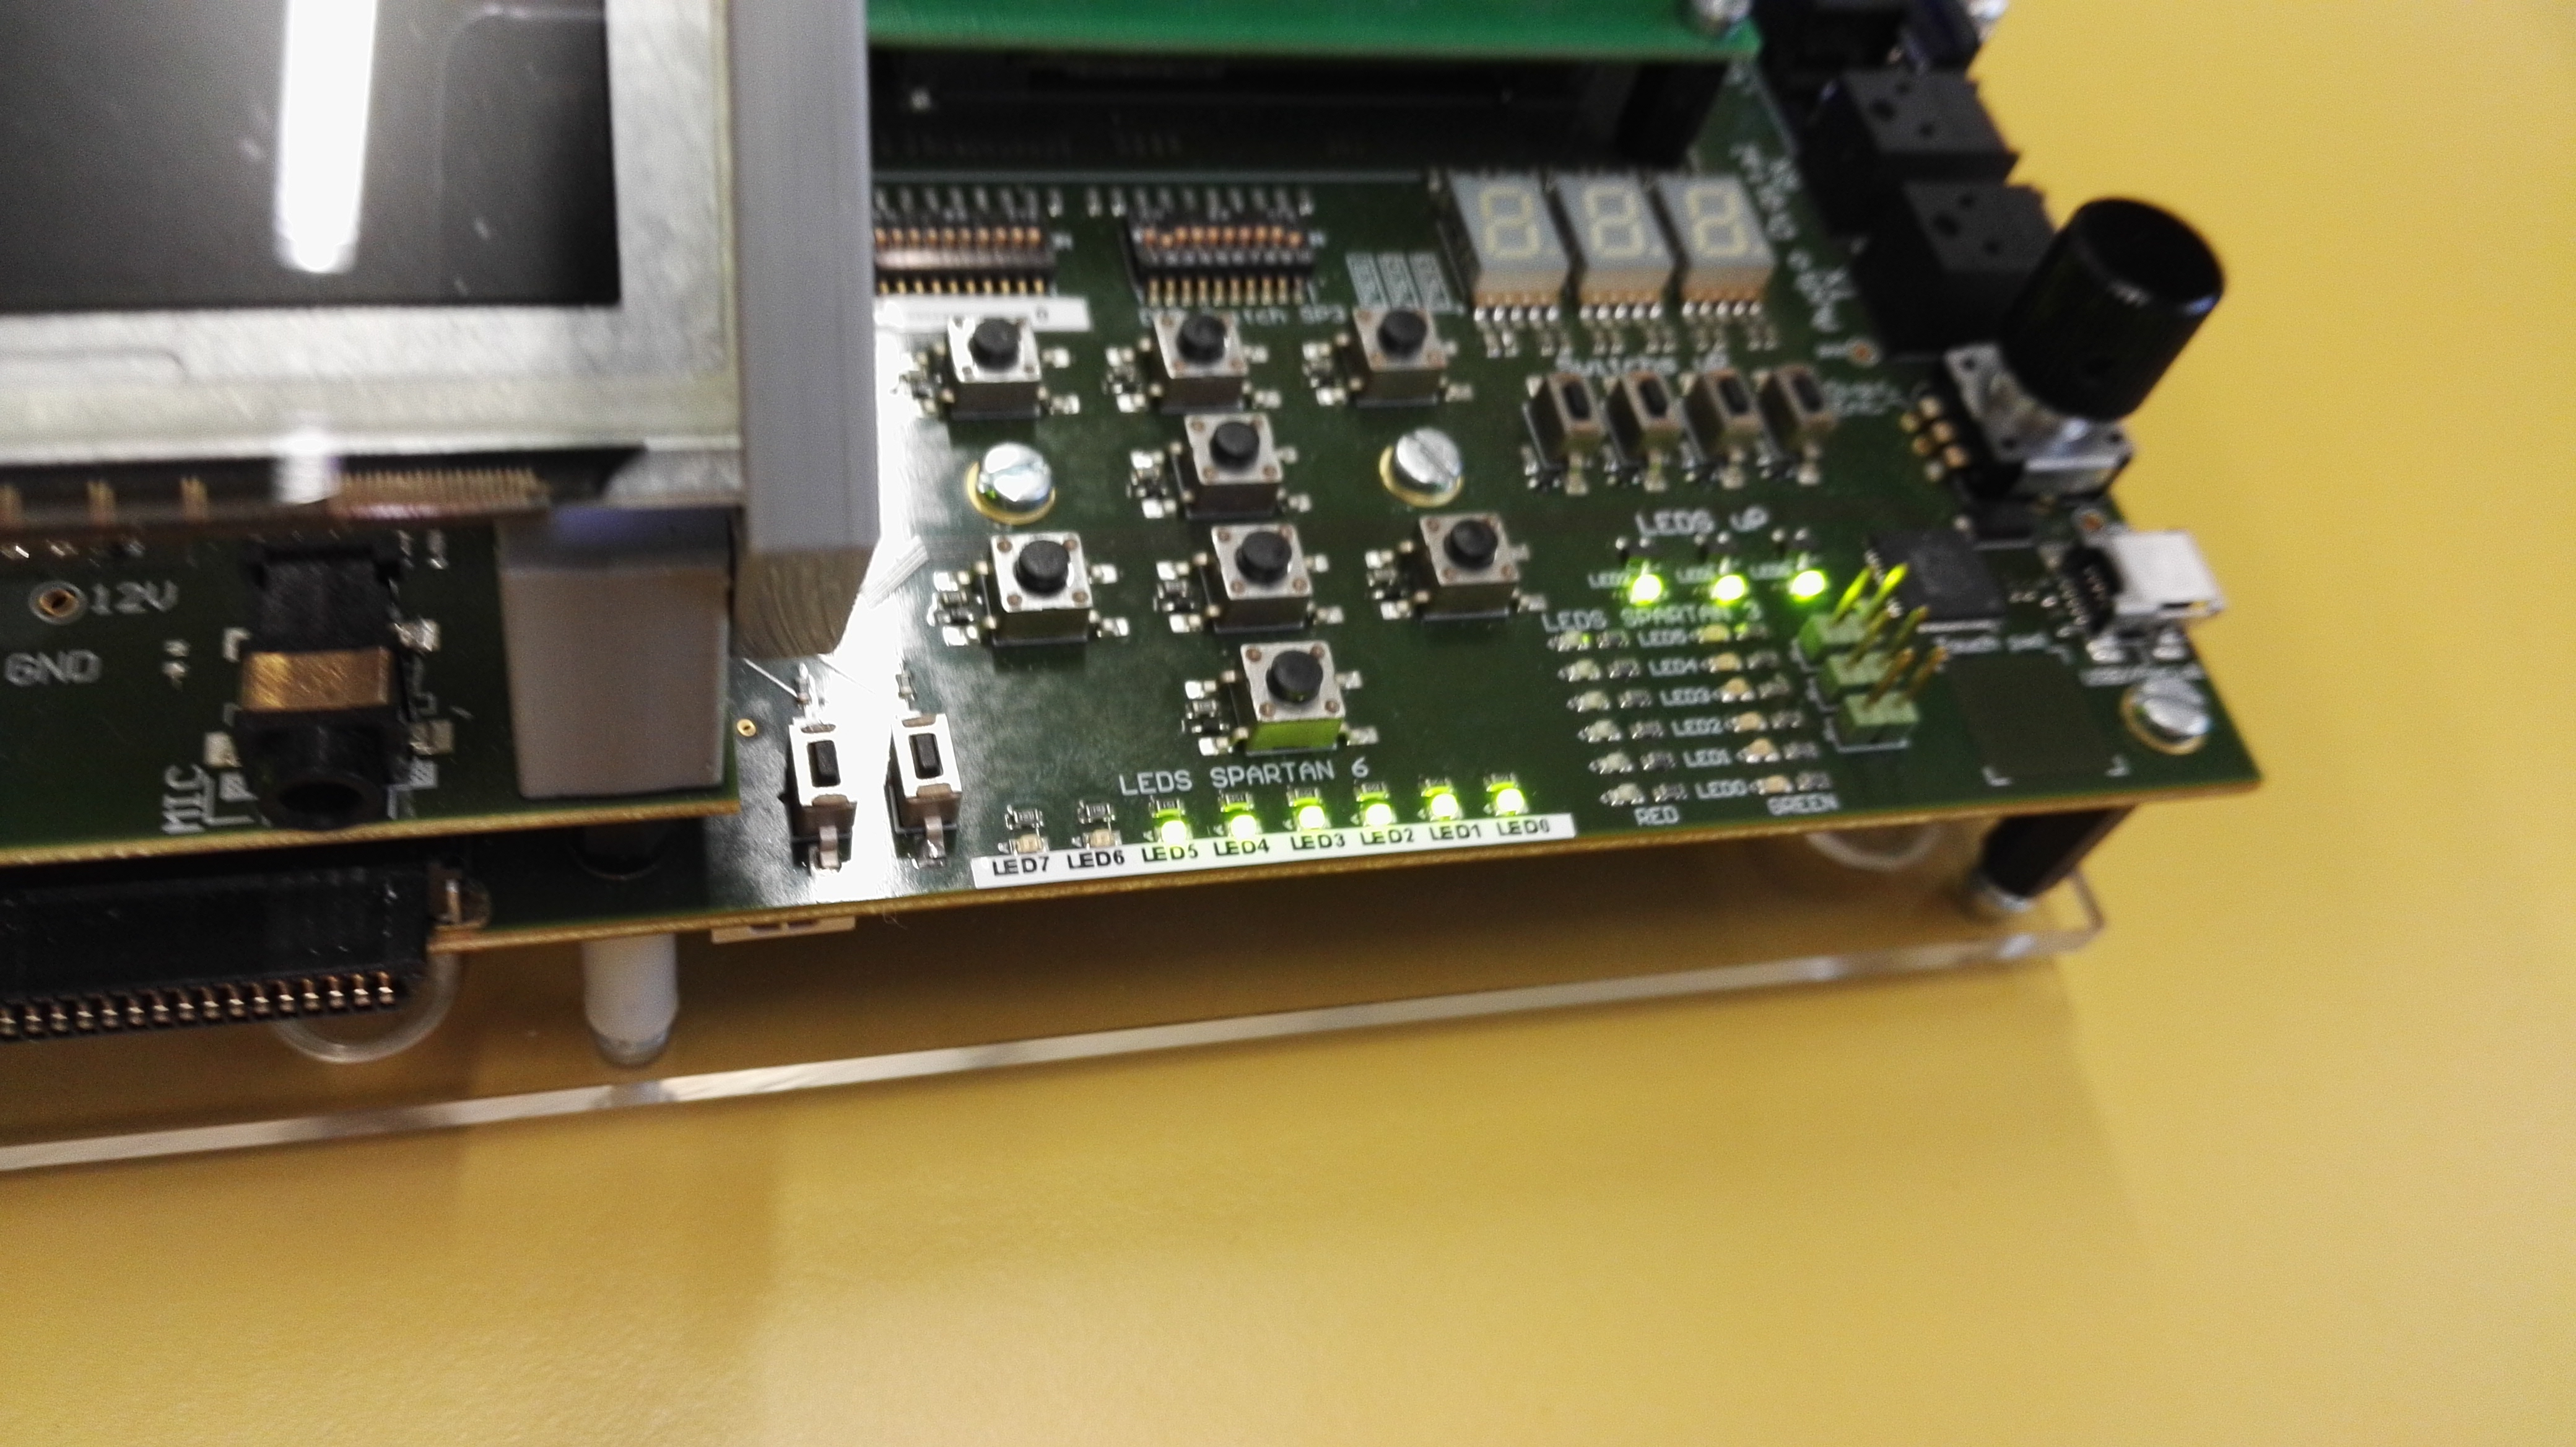
\includegraphics[width=17cm]{img/driverLeds3.png}
		\caption{Allumage des LEDs}
		\label{driverLed2}
	\end{center}
\end{figure}
\begin{figure}[H]
	\begin{center}
		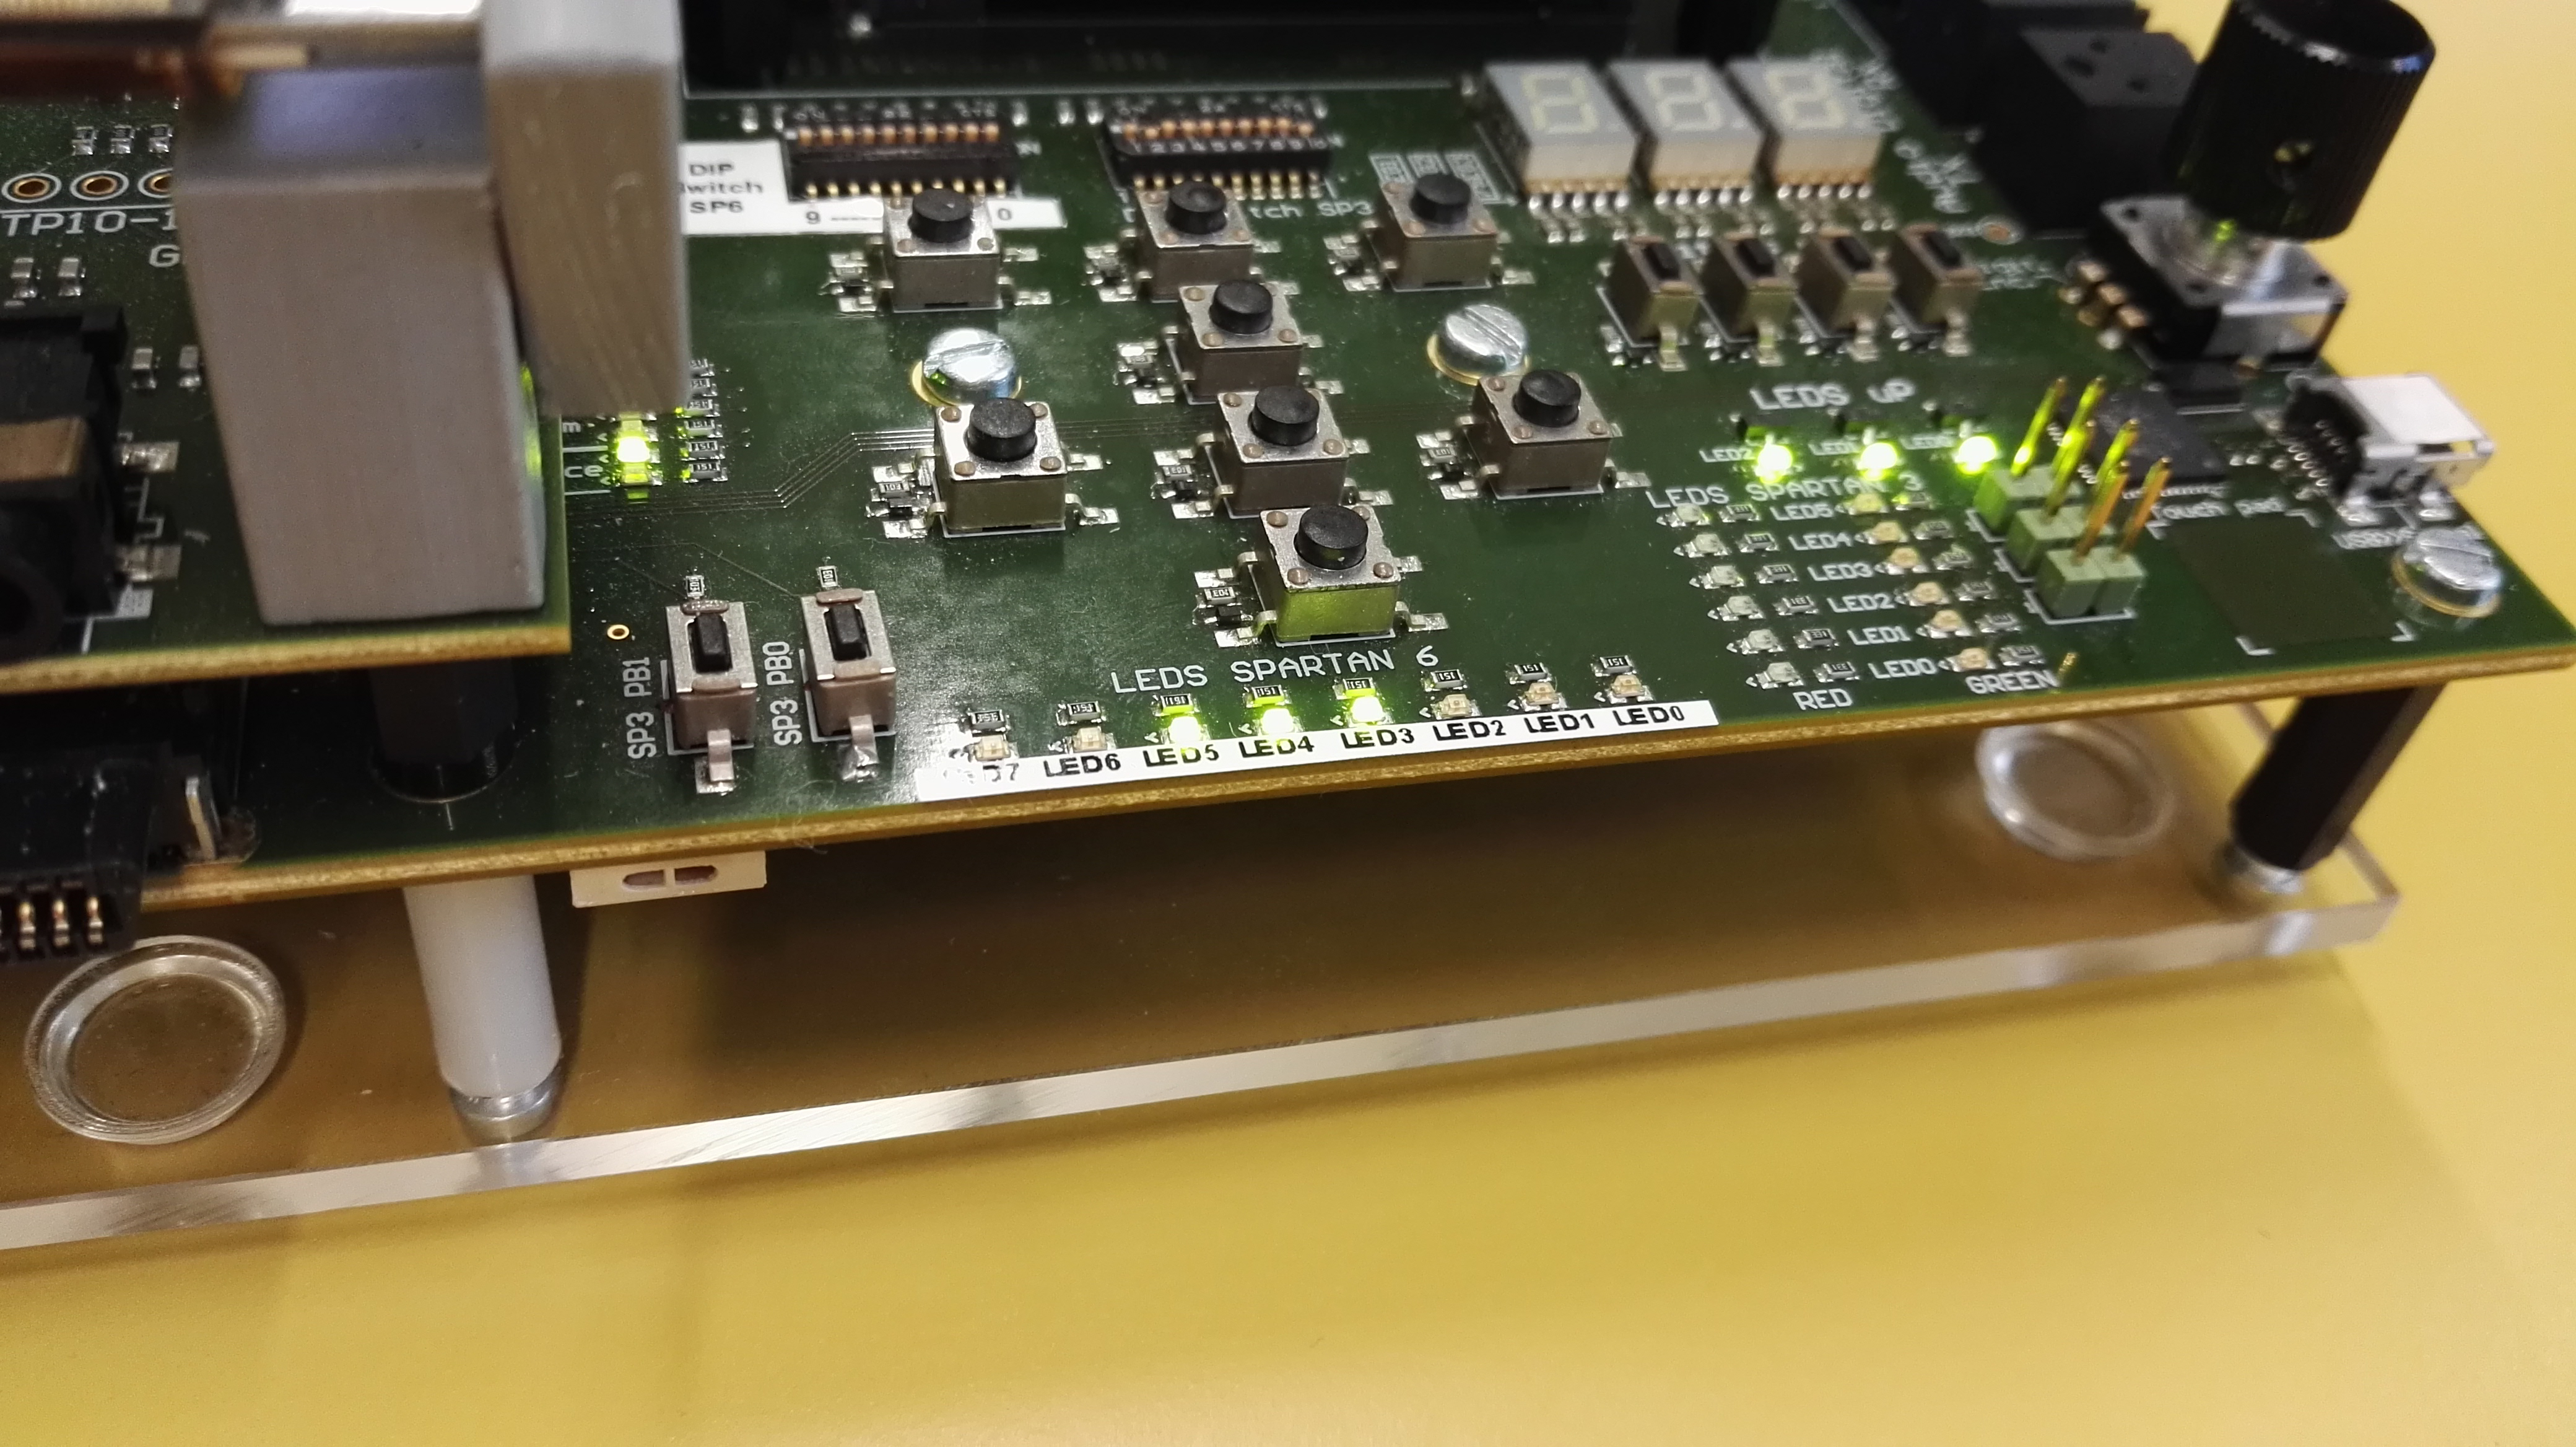
\includegraphics[width=17cm]{img/driverLeds2.png}
		\caption{Extinction des LEDs}
		\label{driverLed}
	\end{center}
\end{figure}
\color{red}\subsection{Pilotage des boutons}
Lors de cette étape, nous travaillerons sur le driver gérant la pression des boutons. L'objectif est de
contrôler une application dans l'espace utilisateur à l'aide des boutons.\\\\
\textbf{a) Donnée: }Complétez la fonction probe( ) pour l'enregistrement des deux callbacks d'interruption (traitement
immédiat + traitement différé) à l'aide de la fonction request\_threaded\_irq().\\\\
\textbf{Travail réalisé: }\\\\
\textbf{b) Donnée: }Implémentez le traitement immédiat lié à l'interruption. Il devra :
\begin{enumerate}
	\item stocker la valeur du registre bouton dans le champ current\_button de la structure privée
	(l'adresse du registre contenant cette information est également disponible dans la structure
	privée)
	\item acquitter l'interruption.\\
\end{enumerate}
\textbf{Travail réalisé: }\\\\
\textbf{c) Donnée: }Testez votre driver boutons à l'aide de l'application buttons\_test. Dans l'environnement émulé,
l'application devra ouvrir le fichier /dev/input/event1. Il faudra taper la commande suivante:
\begin{lstlisting}
# ./buttons_test -e1
\end{lstlisting}
Testez les boutons un par un.\\\\
\textbf{Travail réalisé: }\\\\
\textbf{d) Donnée: }Testez votre driver avec une application Qt disponible dans /usr/share/qt/demos. Essayez textedit
par exemple : 
\begin{lstlisting}
# export QWS_KEYBOARD="LinuxInput:/dev/input/event1"
# cd /usr/share/qt/demos/textedit
# ./textedit -qws 
\end{lstlisting}
\textbf{Travail réalisé: }\\\\
\textbf{e) Donnée: }Effectuez un déploiement et un test sur la plate-forme réelle Reptar. Sur la plate-forme réelle, vous
devrez utiliser l'entrée /dev/input/event2
\textbf{Travail réalisé: }\\\\
\textbf{Réponse aux questions: }A la fin de cette étape, vous devrez être en mesure de décrire le cheminement d'une interruption
en provenance d'un bouton jusqu'à l'effet perçu au niveau de l’application utilisateur. \\\\
\textbf{Travail réalisé: }\\\\\color{black}